\documentclass[notitlepage]{revtex4-1}
%\documentclass[preprint]{revtex4-1}
%\documentclass[preprint,draft]{revtex4-1}

\usepackage{graphicx}
%\usepackage{fancyhdr}
%\usepackage{authblk}
%\usepackage{natbib}

% Set up headers and footers
%\pagestyle{fancy}

\def\myeqnum#1{(\ref{eq:#1})}
\def\eq#1{Eq.~\myeqnum{#1}}
\def\eqs#1{Eqs.~\myeqnum{#1}}
\def\eqn#1{\myeqnum{#1}}
\def\figref#1{Fig.~\ref{fig:#1}}

\newcommand{\matlab}{{\sc Matlab}}
\newcommand{\ud}{\mathrm{d}}

% Put any new macros here

\begin{document}

\title{Mass spectrometry analysis software}

\author{Timothy E. Holy}
% \altaffiliation{To whom correspondence should be addressed}
\affiliation{Department of Anatomy \& Neurobiology, Washington University School of Medicine, St. Louis, Missouri}


%\lhead{\emph{Running head}}
%\chead{}
%\rhead{\thepage}
%\lfoot{}
%\cfoot{}
%\rfoot{}

\date{\today}

%\begin{abstract}
%Here's the abstract
%\end{abstract}

\maketitle

This document contains some description of the mass spectrometry analysis suite, along with recommendations on how to use it.


\section{Getting started}

First load your data:
\begin{verbatim}
>> scan = msload_mzXML('myfile.mzXML');
\end{verbatim}
If you get errors, this likely stems from certain assumptions I've made about the mzXML format (which I deduced simply by looking at a few files we had in hand, and may therefore reflect idiosyncracies of a specific instrument).  %Now that \matlab\ can import mzXML, it might be possible to convert their format to my format (which is necessary for using the downstream code).

For reference, the \verb|scan| structure has the following appearance:
\begin{verbatim}
>> scan

scan = 

1x2376 struct array with fields:  % one element for each separate scan
    scan_time  % the time at which the given scan occurred (seconds)
    ms_level   % level 1 = "direct", level 2 = MS/MS, level 3 = MS^3, etc.
    min_mz
    max_mz
    totIntensity
    precursor_mz  % this and next filled in if this scan is MS/MS or higher
    precursor_I
    n_points
    mz
    intensity
\end{verbatim}
An example:
\begin{verbatim}
>> scan(1)

ans = 

       scan_time: 0.7042
        ms_level: 1
          min_mz: 80.0003
          max_mz: 1.2020e+03
    totIntensity: 486058
    precursor_mz: NaN
     precursor_I: NaN
        n_points: 5987
              mz: [1x5987 single]
       intensity: [1x5987 single]
\end{verbatim}
The most important data are the fields \verb|mz| and \verb|intensity|; \verb|scan(i).intensity(j)| is a measure of the ion current recorded at an $m/z$ of \verb|scan(i).mz(j)| during the $i$th scan.  Note this is a ``sparse'' storage format, i.e., $m/z$ values with below-threshold intensity (``zero'' intensity) are not listed.

You should also look at your data:
\begin{verbatim}
>> msbrowse(scan)
\end{verbatim}
This will open up 3 windows, of which the ``main'' window will look like this:
\begin{center}
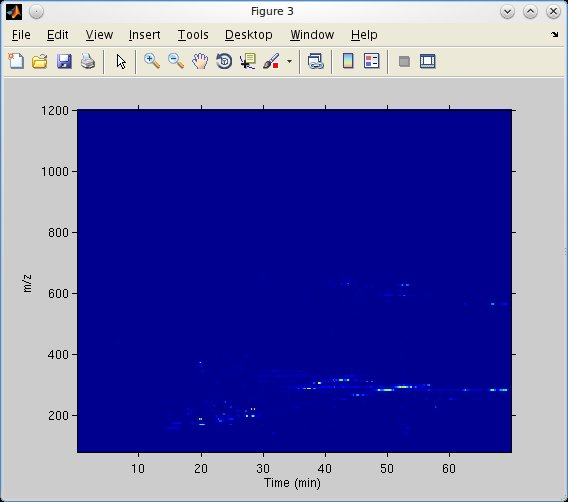
\includegraphics[width=4in]{figures/browse_mainwindow}
\end{center}
This is a plot of intensity as a function of elution time and $m/z$.  You can zoom in/out, get time-slice data, and even see the MS/MS results.  See the help for \verb|msbrowse| for more information.

\section{Adding gradient information}

One of the first things you'll want to do is supply information about the solvent gradient.  If you want to do this,
 create a file (in the same directory as the raw data) with the name
\verb|set_gradients.m|.  The syntax of this function should be \verb|gc = set_gradients(flc)|,  where \verb|flc| is a cell array of file names and the output \verb|gc| is a cell array, each entry giving the gradient supplied for the
     corresponding file in \verb|flc|.

 The syntax of gradient information is the following:
\begin{verbatim}
    [t1    c1; ...
     t2    c2; ...
     t3    c3; ...
     ...]
\end{verbatim}
 where \verb|ci| is the \%B at time \verb|ti|.  Between the times in this table, the concentration is linearly
 interpolated; you need to make sure you encode this
 accurately.  For example, suppose you start at 10\%B, hold there for 5
 minutes, then ramp up to 80\%B over 15 minutes, then hold it for the
 next 10 minutes, then drop back down to 10\%B over 2 minutes.  This
 would be supplied as
\begin{verbatim}
    [0 10;
     5 10;
     20 80;
     30 80;
     32 10];
\end{verbatim}
 You really should plot this information to check that you've gotten it
 right, e.g., \verb|plot(m(:,1),m(:,2))|.

Once this file has been added to the data directory (and is on the \matlab\ path), you should automatically get gradient information attached.  If you see a warning, ``Gradient data not available,'' then something is wrong.


\section{Quantifying abundance across samples}

Here I'm assuming you have one or more LC/MS scans collected in profile mode, and you want to quantify abundance of the individual peaks, perhaps across samples.

The getting-started function is \verb|msprof_extract_compounds_set|.  As a warning, thus function has by far the most annoyingly-primitive interface of all of them; the only saving grace is that the amount of time you spend using this function interactively is small.  You can start it quite simply typing \verb|msprof_extract_compounds_set|.  This file has some fairly lengthy help, and you are referred to that for direct assistance.  Here I will describe what the core of this analysis is doing.

The main idea is to \emph{factor} the ion abundance data into components.  Let $I(y,t)$ represent the abundance of an ion of $m/z = y$ eluting at time $t$.  Each compound in this sample will have an $m/z$ profile, meaning that if you averaged over time, you would see a peak in the $m/z$ spectrum (for a high-resolution instrument this peak will be quite narrow, but will still span multiple $m/z$ values; the commonly-quoted $m/z$ corresponds to peak or average $m/z$).  The shape of this peak might be described as $M(y)$.  It will also have an elution profile over time, corresponding to a temporal abundance of $T(t)$.  The idea is to decompse $I(y,t)$ like this:
\begin{equation}
I(y,t) \approx \sum_i M_i(y) T_i(t),
\end{equation}
where each $i$ corresponds to a different peak (with presumably different peak $m/z$ and different temporal elution profile).  That is, we try to explain the observed data as a sum of independent peaks.  In particular, since no compound can have negative abundance, $I$, $M_i$, and $T_i$ should all be nonnegative, and thus this is nonnegative matrix factorization (NNMF).

I spent some time trying ``canned'' NNMF routines, and my conclusion is that for this problem they do not work.  There are two problems:
\begin{itemize}
\item You have to specify in advance how many components you want.  For MS data, this may not be known.
\item A simultaneous fit for thousands of components takes a long time and rarely separates individual compounds into separate components.
\end{itemize}
However, by imposing something that we know---a given compound has a narrow range of $m/z$ to which it contributes intensity---one can easily come up with a custom sequential NNMF algorithm:
\begin{enumerate}
\item Start with the biggest peak across all $m/z$
\item \label{item:factor} Explain this peak (looking at just a narrow range of $m/z$ values around the peak) as a product $M(y) T(t)$ (this is a straightforward alternating optimization problem, see the code)
\item Use the $T(t)$ as the temporal component to fit the $\tilde M(y)$ profile of the common isotopologues; extract an estimate of the abundance of each isotopologue as well as an estimate of the charge (which you can deduce by looking for a $^{13}$C isotopologue at $\Delta m/q$, where $q$ is the integer charge and $\Delta m$ is the mass difference between $^{12}$C and $^{13}$C).
\item Blank the portion of $I(y,t)$ that is covered by this peak and its isotopologues
\item Find the biggest-remaining peak
\item Go back to step \#\ref{item:factor}; only quit when you get down into the noise.
\end{enumerate}
\emph{One word of warning}: the implementation currently assumes that the most abundant isotopologue is also the lowest-mass isotopologue.  This makes it unsuitable for large ions, like proteins.  This assumption could, with a bit of effort, be relaxed, but for the small molecules we care about I do not think this is a problem.

The NNMF step is the most useful and powerful component of the calculation.  Following the completion of the NNMF step, there is one more step:  an attempt to automatically identify temporal peaks in the $T_i(t)$.  In my view, this may be a useful step, but I am not yet happy with the job that it does on its own.  It is important to check, and surely modify, some of its decisions by human intervention.  This is described in the next section.

This code will generally run for several hours.  Wait for it to finish.

I should also explain one other detail:  $m/z$ values are converted to an integer index.  This is necessary because, at least for one of the mass specs we use, it seems to scan at very-slightly-different $m/z$ values on different scans, but the discrepancy is much smaller than the resolution of the instrument.  This is a pain, because it prevents you from straightforwardly comparing the ``same'' $m/z$ value on separate scans even within a single file.  So, I decided to ``round off'' these small variations, i.e., convert to an integer index.  I tried to do this quite carefully, in a way that preserves the full resolution of the instrument---analyzing the data on our instrument, I found that the $m/z$ accuracy is approximately logarithmic (i.e., follows Weber's law), but not precisely.  So I fit $\Delta m/z$ (the gap in $m/z$ between adjacent mass values) to a quadratic. \matlab\ prefers to do this in terms of a centered and scaled version of $m/z$, i.e.,
\begin{equation}
x = \frac{m/z - \mu_1}{\mu_2},
\end{equation}
where \verb|polyfit| it will supply the values of $\mu_1$ and $\mu_2$.  Then we define a integer index function ${\cal I}(m/z)$ such that
\begin{equation}
{\cal I}(m/z + \Delta m/z) - {\cal I}(m/z) = 1,
\end{equation}
i.e.,
\begin{equation}
\ud {\cal I} = \frac{\ud (m/z)}{\Delta m/z} = \mu_2 \frac{\ud x}{ax^2+bx+c},
\end{equation}
where $a$, $b$, and $c$ are the parameters of the quadratic fit.  Thus
\begin{equation}
{\cal I}(x) = \mu_2 \int_{x_\mathrm{min}}^x \frac{\ud x'}{ax'^2+bx'+c}.
\end{equation}
This integral is performed in Gradshteyn \& Rhyzik (2.172, 5th edition).  (The only subtlety is that the polynomial sometimes has complex roots.)
I also do linear interpolation on the measured intensity, so there aren't any ``holes'' in the output due to rounding.

It should also be pointed out that the data stored in the \verb|nnmf| file may be of intrinsic interest; you could easily write your own functions to extract quantities of particular interest to you.  Here is an explanation of the information in this file:

\begin{verbatim}
>> s = load('msprof_ecs_nnmf.mat')

s = 

            file: {1x3 cell}                                % The list of files
            mz2i: @(mz)mz2indx_fun(mz,p(1),xr,mu,xmin)      % a function handle: m/z -> integer index
            i2mz: @(i)indx2mz_fun(i,p(1),xr,mu,xmin)        % a function handle: integer index -> m/z
              tc: {[1x367 double]  [1x360 double]  [1x361 double]}  % scan times
standardMzIShift: 0                           % registration info, I think
          Mmzmax: [1859370x1 double]          % the total profile (max projection along the time axis)
     nnmfresults: [1x1000 struct]             % here's the interesting bit
         randKey: 0.8147                      % for ensuring this file is in sync with others

\end{verbatim}

The \verb|nnmfresults| variable looks like this:
\begin{verbatim}
>> s.nnmfresults

ans = 

1x1000 struct array with fields:
    mzMeanCorrected
    totIntensity
    mzCorrected
    mzProf
    iProf
    iProfBlank
    nnmf_err
    Mmzrange
    charge
    chargeI
    nI
    nIcov

>> s.nnmfresults(1)

ans = 

    mzMeanCorrected: 296.2574   % the "m/z" of the compound (corrected for any registration error)
       totIntensity: 3.7951e+10           % total across all samples
        mzCorrected: [1x11 double]        % ?
             mzProf: [11x1 double]        % The peak profile in m/z
              iProf: {[1x367 double]  [1x360 double]  [1x361 double]}
         iProfBlank: []                   % The standard sample
           nnmf_err: 3.5261e+17           % NNMF fitting error
           Mmzrange: [1242482 1242492]    % integer index of m/z range
             charge: 1                    % ion charge (sign is not preserved)
            chargeI: [5.0386e+12 6.3702e+14 2.2319e+11 2.4703e+18]
                 nI: [62.1759 19.0530 1.5348 -0.0019 0.0015 NaN]
              nIcov: [6x6 double]

\end{verbatim}
Notes:
\begin{itemize}
\item \verb|iProf|:    The elution profile in time, for all samples
\item \verb|chargeI|:   raw data used to assign the charge; \verb|chargeI(end)| had better really dominate if \verb|charge| is 1, \verb|chargeI(end-1)| should dominate if \verb|charge| is 2, and so on. If nothing sticks out, don't trust the charge.
\item \verb|nI|:     Estimate of abundance of particular atoms based on isotopologues; the order is whatever you supplied for \verb|isotopeoptions| (default H, C, O, S, N, P)
\item \verb|nIcov|:   Estimate of the covariance matrix for the fit that determined nI. This is \emph{normalized}, so the absolute magnitude is meaningless (because we don't have an estimate for the uncertainties in the intensity).  But relative error might be useful.
\end{itemize}

The order of entries in nnmfresults is in decreasing abundance.

\section{Inspecting/modifying the factoring result}

There is a much friendlier GUI for examining the results:  \verb|msprof_choose_peak_timecourses_gui|.  This too can be run from the command line without any arguments.

Here is a screenshot:
\begin{center}
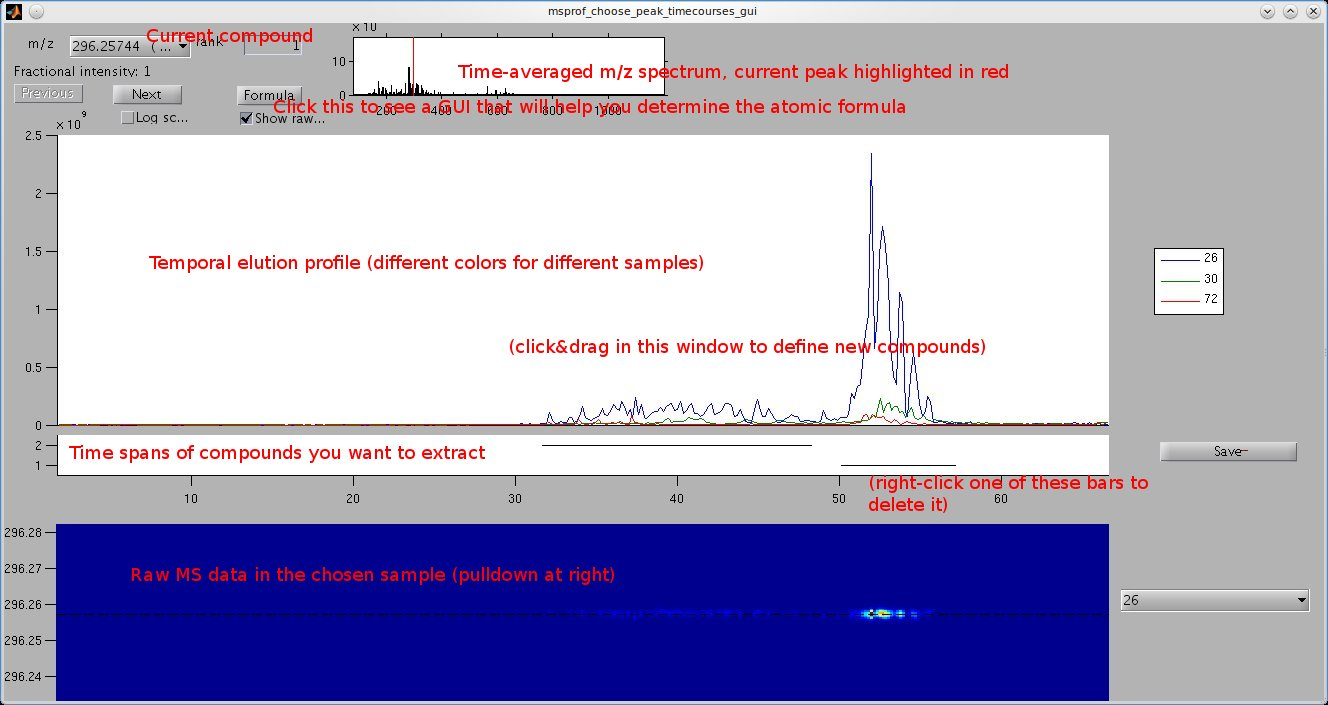
\includegraphics[width=6in]{figures/choosepeakGUI_edit.jpeg}
\end{center}
The labels in red are superimposed to explain the important components of this window; you will not see them in the actual window.

Note that the ``compounds'' identified by a bar have multiple peaks; this might mean that one of both of these actually consists of multiple compounds that elute in close succession.  One of the clearest signatures of different compounds occurs when the intensity is modulated differently in different samples.  I often tend to ``lump'' unless there is clear evidence that things need to be separated.

You can modify the timespans as instructed in the help for \verb|msprof_choose_peak_timecourses_gui|.  Any changes are saved to the original \verb|compounds| file.

Here is the formula GUI:
\begin{center}
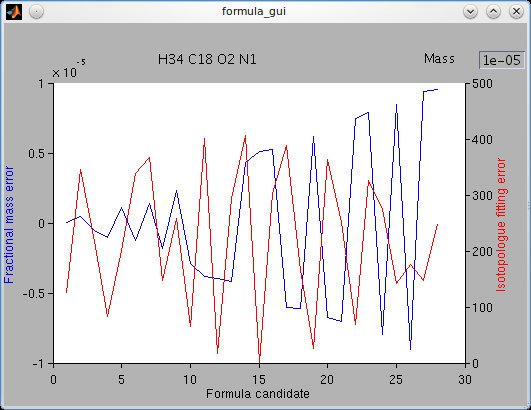
\includegraphics[width=3.5in]{figures/formulaGUI}
\end{center}
The blue line plots the mass error; the red line plots the error in fitting the \verb|nI| data described above (weighted by the inverse of the covariance matrix \verb|nIcov|).  Click on a point that has not-too-large mass error and small \verb|nI|-fitting error.  The corresponding formula will be shown above.  You can often rule out some formulas as being implausible by their C-to-H ratio or by using the rule of nitrogen.  Obviously, the accuracy of the isotopologue fitting goes down for lower-abundance peaks, so for very small peaks you should not take this seriously.


\section{Final step: extracting the concentrations across samples}

A final (and quite simple) program, \verb|msprof_concentrations|, will calculate the estimated concentration of each peak in each sample for which you have drawn a ``bar'' to define a temporal range.  See its help for details.

\end{document}
